\documentclass{beamer}
\usepackage[czech]{babel}

\usetheme[fei,sign]{vsb}

\title[Simulace Turingova stroje strojem RAM]{Simulace Turingova stroje strojem RAM}
% \subtitle{Simulace Turingova stroje RAMem}
\author{Bc. Jakub Koběrský}
% \institute[VŠB-TUO]{VŠB -- Technická univerzita Ostrava\\\vspace{2mm}jmeno.prijmeni@vsb.cz}
\date[15.~3.~2025]{15.~března 2025}

\showboxdepth=5

\begin{document}

%\begin{frame}
%	\tableofcontents
%\end{frame}

% Úvod - cíl, motivace
% Popis simulace
% Funkce
% UI
% Závěr - případy použití, zhodnocení, možné rozšíření

\section{Úvod}
\begin{frame} 
\setbeamercovered{invisible}
	\frametitle{Cíle práce}
	\uncover<1->{\textbf{Cíl}}
	\begin{itemize}
		\item<1-> Komponentu pro simulaci Turingova stroje RAMem
	\end{itemize}
    \bigskip
    \uncover<1->{\textbf{Zadání práce}}
    \begin{enumerate}
        \item<1-> Komponenta pro výuku teoretické informatiky
        \item<1-> Možnost zadání vlastní specifikace Turingova stroje
        \item<1-> Současná simulace výpočtu strojů
        \item<1-> Předpřipravené vstupy
    \end{enumerate}
\end{frame}

\section{Teorie}
\begin{frame} 
	\setbeamercovered{invisible}
	\frametitle{Inicializace stroje RAM}
    \textbf{Vstup}: instance Turingova Stroje
    \begin{enumerate}
        \item Vytvoření slovníku/legendy
        \item Vytvoření kódu stroje RAM
        \begin{itemize}
            \item Načtení vstupní pásky do paměti \& inicializace
            \item Pro všechny stavy... 
            \item Pro stavy se symbolem...
            \item Výpis na výstupní pásku
        \end{itemize}
        \item Enkódování pásky TS a vložení na vstup RAM
        \item Inicializace stroje RAM
    \end{enumerate}
	
\end{frame}

\section{Teorie}
\begin{frame}
	\frametitle{Vývoj}
    \begin{itemize}
        \item Webová aplikace přes React.js, běží lokálně
        \item Každý stroj dědí ze třídy \texttt{Machine}
        \begin{itemize}
            \item Shodné chování mezi stroji
            \item Jednodušší zpracování chyb
            \item Simulace brána jako samostatný stroj
        \end{itemize}
    \end{itemize}
    \bigskip
    \begin{center}
        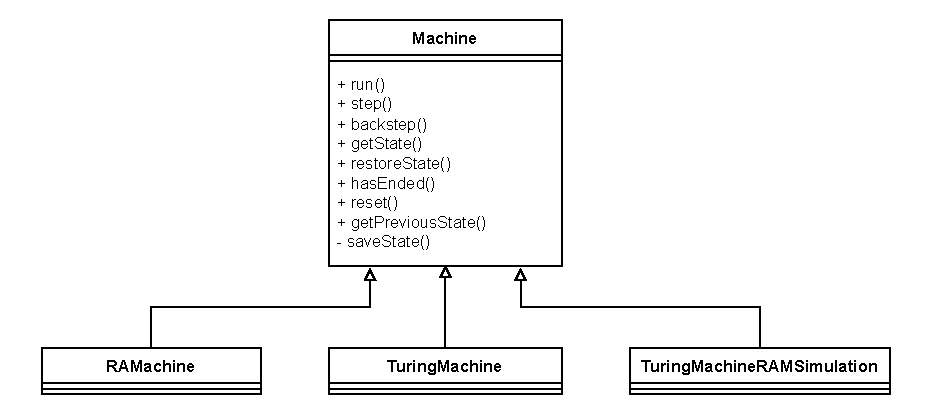
\includegraphics[height=0.5\textheight]{fig/class_diagram.drawio.pdf}
    \end{center}
\end{frame}

\section{Teorie}
\begin{frame}
	\frametitle{Funkce}
    \begin{itemize}
        \item Implementace stroje RAM a TS
        \item Implementace simulace
        \item Předpřipravené definice TS, vytvoření nové, import
        \item Krokování podle TS i RAM
        \item Automatický běh simulace
        \item Animace simulace
    \end{itemize}
\end{frame}

\section{Ukázka}
\begin{frame}
	\frametitle{Seznam definic}
    \begin{center}
        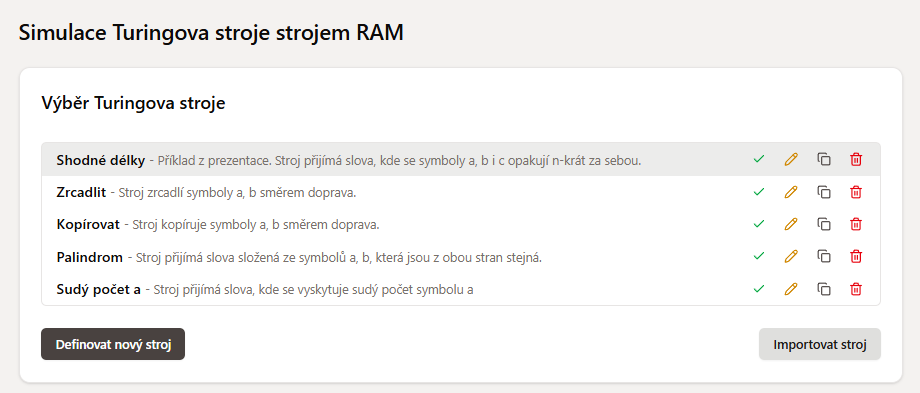
\includegraphics[height=0.5\textheight]{fig/obr1.png}
    \end{center}
\end{frame}

\section{Ukázka}
\begin{frame}
	\frametitle{Nová definice}
    \begin{center}
        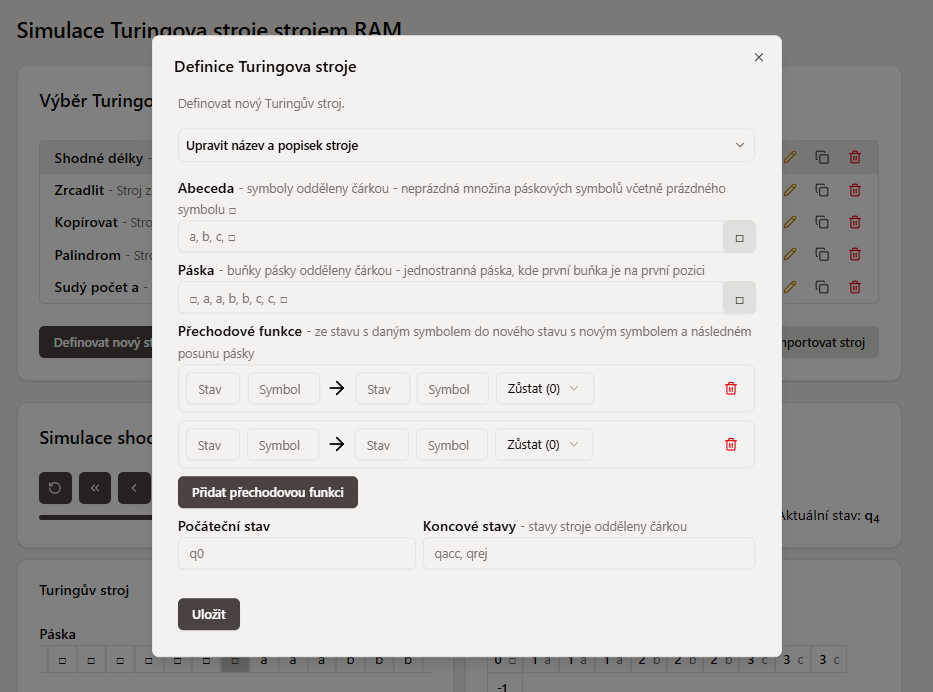
\includegraphics[height=0.85\textheight]{fig/obr2.png}
    \end{center}
\end{frame}

\section{Ukázka}
\begin{frame}
	\frametitle{Prostor simulace}
    \vspace{-2.6mm}
    \begin{center}
        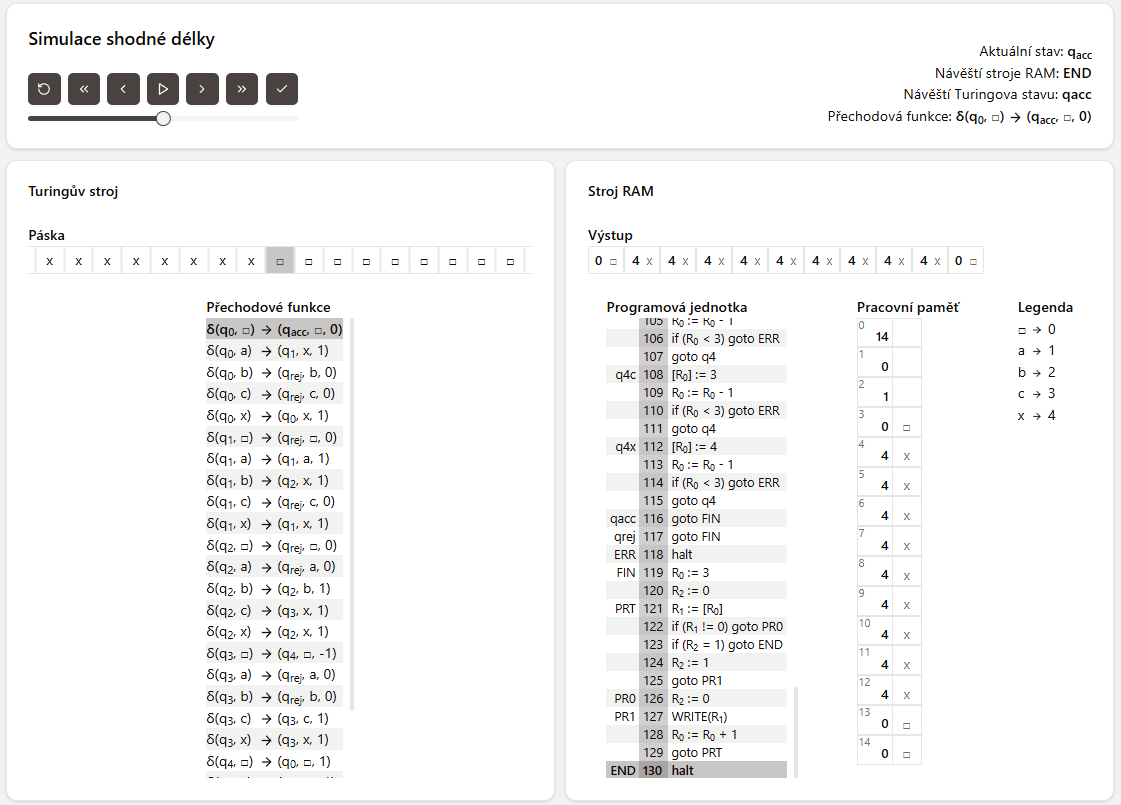
\includegraphics[height=0.913\textheight]{fig/obr4.png}
    \end{center}
\end{frame}

\section{Ukončení}
\begin{frame}
	\frametitle{Závěr}
	\uncover<1->{\textbf{Případy použití}}
	\begin{itemize}
		\item<1-> Komponenta pro výuku
	\end{itemize}
    \bigskip
    \uncover<1->{\textbf{Zhodnocení}}
    \begin{itemize}
		\item<1-> Jednoduché na použití
	\end{itemize}
    \bigskip
    \uncover<1->{\textbf{Možné rozšíření}}
    \begin{itemize}
		\item<1-> Podpora jazyků
        \item<1-> Více variant strojů
        \item<1-> Offline režim
	\end{itemize}
    \bigskip
    \bigskip
    \uncover<1->{Dostupné na adrese \texttt{https://ram.koberskyj.cz}}
\end{frame}

\section{Ukončení}
\begin{frame}
	\frametitle{Konec}

    \bigskip
    \bigskip
    \bigskip
    \bigskip
    \bigskip
    \bigskip
    \begin{center}
        \textbf{Děkuji za pozornost}
    \end{center}
    \bigskip
    \bigskip
    \bigskip
    \bigskip
    \bigskip
    \bigskip
    Dostupné na adrese \texttt{https://ram.koberskyj.cz}
\end{frame}

\end{document}
